% Chapter 5

\chapter{Cloudlets} % Main chapter title

\label{ch:Chapter4} % For referencing the chapter elsewhere, use \ref{Chapter1} 

\lhead{Capítulo 4. \emph{Cloudlets}} % This is for the header on each page - perhaps a shortened title

%----------------------------------------------------------------------------------------

Con la ayuda de la nube, los dispositivos móviles pueden migrar las partes computacionalmente intensivas de sus aplicaciones. Los `inacabables' 
recursos de la nube pueden minimizar los costos de tiempo y energía de las aplicaciones móviles. Sin embargo, como se describió en la sección
\ref{ch:Chapter4}, uno de los aspectos que interfieren realizar \textit{offloading} a la nube es la alta latencia entre la conexión entre el móvil 
y la nube. Adicionando un cloudlet ~\cite{5280678} (una computadora local que provee de 100 a 1000 veces más poder computacional que un dispositivo móvil con 
mínima latencia), crea las posibilidades para ejecutar aplicaciones sensibles a la latencia y que demanden gran poder computacional de un dispositivo
móvil. La noción de \textit{cloudlet} fue introducida como solución a los obstáculos técnicos descritos anteriormente. La idea 
principal es proveer recursos abundantes que son necesitados por los dispositivos móviles no desde una \textit{nube} distante, sino desde
un \textit{cloudlet} cercano. Satyanarayanan \textit{et al.} resumió las diferencias entre \textit{cloudlet} y \textit{cloud}, las cuales están
listadas en la tabla \ref{tab:mainDifferencescloudletcloud}. Se debe notar que el estado flexible sugiere que las copias de cache, datos 
o código están en el dispositivo móvil o \textit{cloud}. En tanto, el estado rígido se refiere a que existe solo una única copia de 
datos o código. Debido a que el \textit{cloudlet} tiene estado flexible, la pérdida de un \textit{cloudlet} no es algo grave. 

%mccarchitecturevscloudlet
% Please add the following required packages to your document preamble:
% \usepackage[table,xcdraw]{xcolor}
% If you use beamer only pass "xcolor=table" option, i.e. \documentclass[xcolor=table]{beamer}
\begin{table}[]
\centering
\caption{Diferencias más notorias entre los entornos \textit{cloudlet} y \textit{cloud} \cite{5280678}}
\label{tab:mainDifferencescloudletcloud}
\begin{tabular}{|l|l|l|}
\hline
\rowcolor[HTML]{EFEFEF} 
               & \multicolumn{1}{c|}{\cellcolor[HTML]{EFEFEF}{\bf Cloudlet}}                                   & \multicolumn{1}{c|}{\cellcolor[HTML]{EFEFEF}{\bf Cloud}}                                                     \\ \hline
Estado         & Solo estado flexible                                                                          & Estado flexible y  rígido                                                                                    \\ \hline
Administración & \begin{tabular}[c]{@{}l@{}}Autogestionado, poca o sin\\  atención profesional\end{tabular}    & Administrado profesionalmente 24/7                                                                           \\ \hline
Entorno        & \begin{tabular}[c]{@{}l@{}}Propiedad descentralizada por \\ los negocios locales\end{tabular} & \begin{tabular}[c]{@{}l@{}}Propiedad centralizada por \\ pocas Empresas (Amazon, Google, etc. )\end{tabular} \\ \hline
Red            & \begin{tabular}[c]{@{}l@{}}Latencia dependiente de la \\ Red de Área Local (LAN)\end{tabular} & \begin{tabular}[c]{@{}l@{}}Latencia de Internet o Ancho de \\ Banda\end{tabular}                             \\ \hline
Escalamiento   & Pocos usuarios a la vez                                                                       & Cientos, Miles o Millones de usuarios a la vez                                                               \\ \hline
\end{tabular}
\end{table}

\subsection{Arquitectura Cloudlet}

Como se describió anteriormente, los \textit{cloudlets} pueden ser usados como intermediarios entre los dispositivos móviles y los servidores 
en la \textit{nube}. Una de las primeras implementaciones de una arquitectura \textit{cloudlet} fue un prototipo de sistema de computación
cloudlet llamado Kimberley~\cite{5280678}, desarrollado por Satyanarayanan \textit{et al.}.  En contraste con la arquitectura en nube, 
Kimberley está conectado a los móviles a través de LAN, no WAN, y es accedido por solamente unos usuarios a la vez. En la Figura
~\ref{fig:mccarchitecturevscloudlet} se 
muestra la arquitectura \textit{cloudlet} en comparación con la arquitectura en nube. El rol principal que cumple un \textit{cloudlet} 
es la administración de tareas. También puede colaborar al dispositivo móvil con algún tipo de procesamiento intermedio.

La arquitectura MOCHA \cite{soyata2013accelerating} (Mobile CLoud Hybryd Architecture) fue creada como una solución a aplicaciones de nube para móviles que requieren
una masiva cantidad de tareas paralelizables. Dicha arquitectura permite que laptops, touchpads, y smartphones se connecten a la nube 
via \textit{cloudlets}, este servicio se realiza usando conexiones de redes múltiples como 3G/4G, Bluetooth, y WiFi. El \textit{cloudlet}
determina como dividir el cálculo entre si mismo y múltiples servidores para optimizar la calidad de servicio (QoS, Quality of Service) 
basado en modelos estadísticos de métricas QoS (latencia, costo monetario, poder de procesamiento, etc.). MOCHA fue demostrado usando 
tareas de reconocimiento de rostros. 
Una arquitectura Similar a Kimberly y a MOCHA, fue propuesta por Ha \textit{et al.}. Esta arquitectura de dos niveles aprovecha un nivel 
de infraestructura en la nube, y un segundo nivel en el borde o \textit{edge} del internet, sirviendo a los dispositivos móviles incorporados 
a la red por medio de WiFi. Los \textit{cloudlets} son pequeños centros de datos próximos al usuario, los cuales solo 
tienen estados flexibles guardados en caché de la nube o de los dispositivos móviles. 
En algunos escenarios como una construcción de oficina, múltiples \textit{cloudlets} pueden estar localizados cerca a otros y pueden estar 
conectados de una forma punto-a-punto. En este caso, la ruta entre entre los móviles, servidores en nube, y los \textit{cloudlets} tiene
que ser tomada en cuenta. En la investigación de Fesehaye \textit{et al.} \cite{6337243} fueron propuestos dos tipos de esquemas de 
enrutamiento o \textit{routing}: centralizado y descentralizado. En el enrutamiento descentralizado la tabla de enrutamiento está 
construida y mantenida por los \textit{cloudlets}. Los \textit{cloudlets} periódicamente emiten información de su presencia a los nodos
vecinos y los otros \textit{cloudlets}. Cuando un dispositivo móvil recibe un mensaje \textit{broadcast} desde un \textit{cloudlet}, 
almacena tal información en una tabla de \textit{cloudlets} adjunto a un identificador (ID) del \textit{cloudlet}. Cada móvil también emite 
periódicamente un mensaje tipo \textit{broadcast} con su identificador, de tal forma que todos los \textit{cloudlets} tengan conocimiento. En 
el enrutamiento centralizado el servidor central es responsable de preparar y mantener la tabla de rutas. El \textit{cloudlet} periódicamente
envía su ID, los ID de sus usuarios móviles y los ID de los \textit{cloudlets} vecinos al servidor central. Consecuentemente, el
servidor central calcula la tabla de rutas para cada \textit{cloudlet} e instala la tabla de reenvíos en todos los \textit{cloudlets}.
\begin{figure}[h]
  \centering
 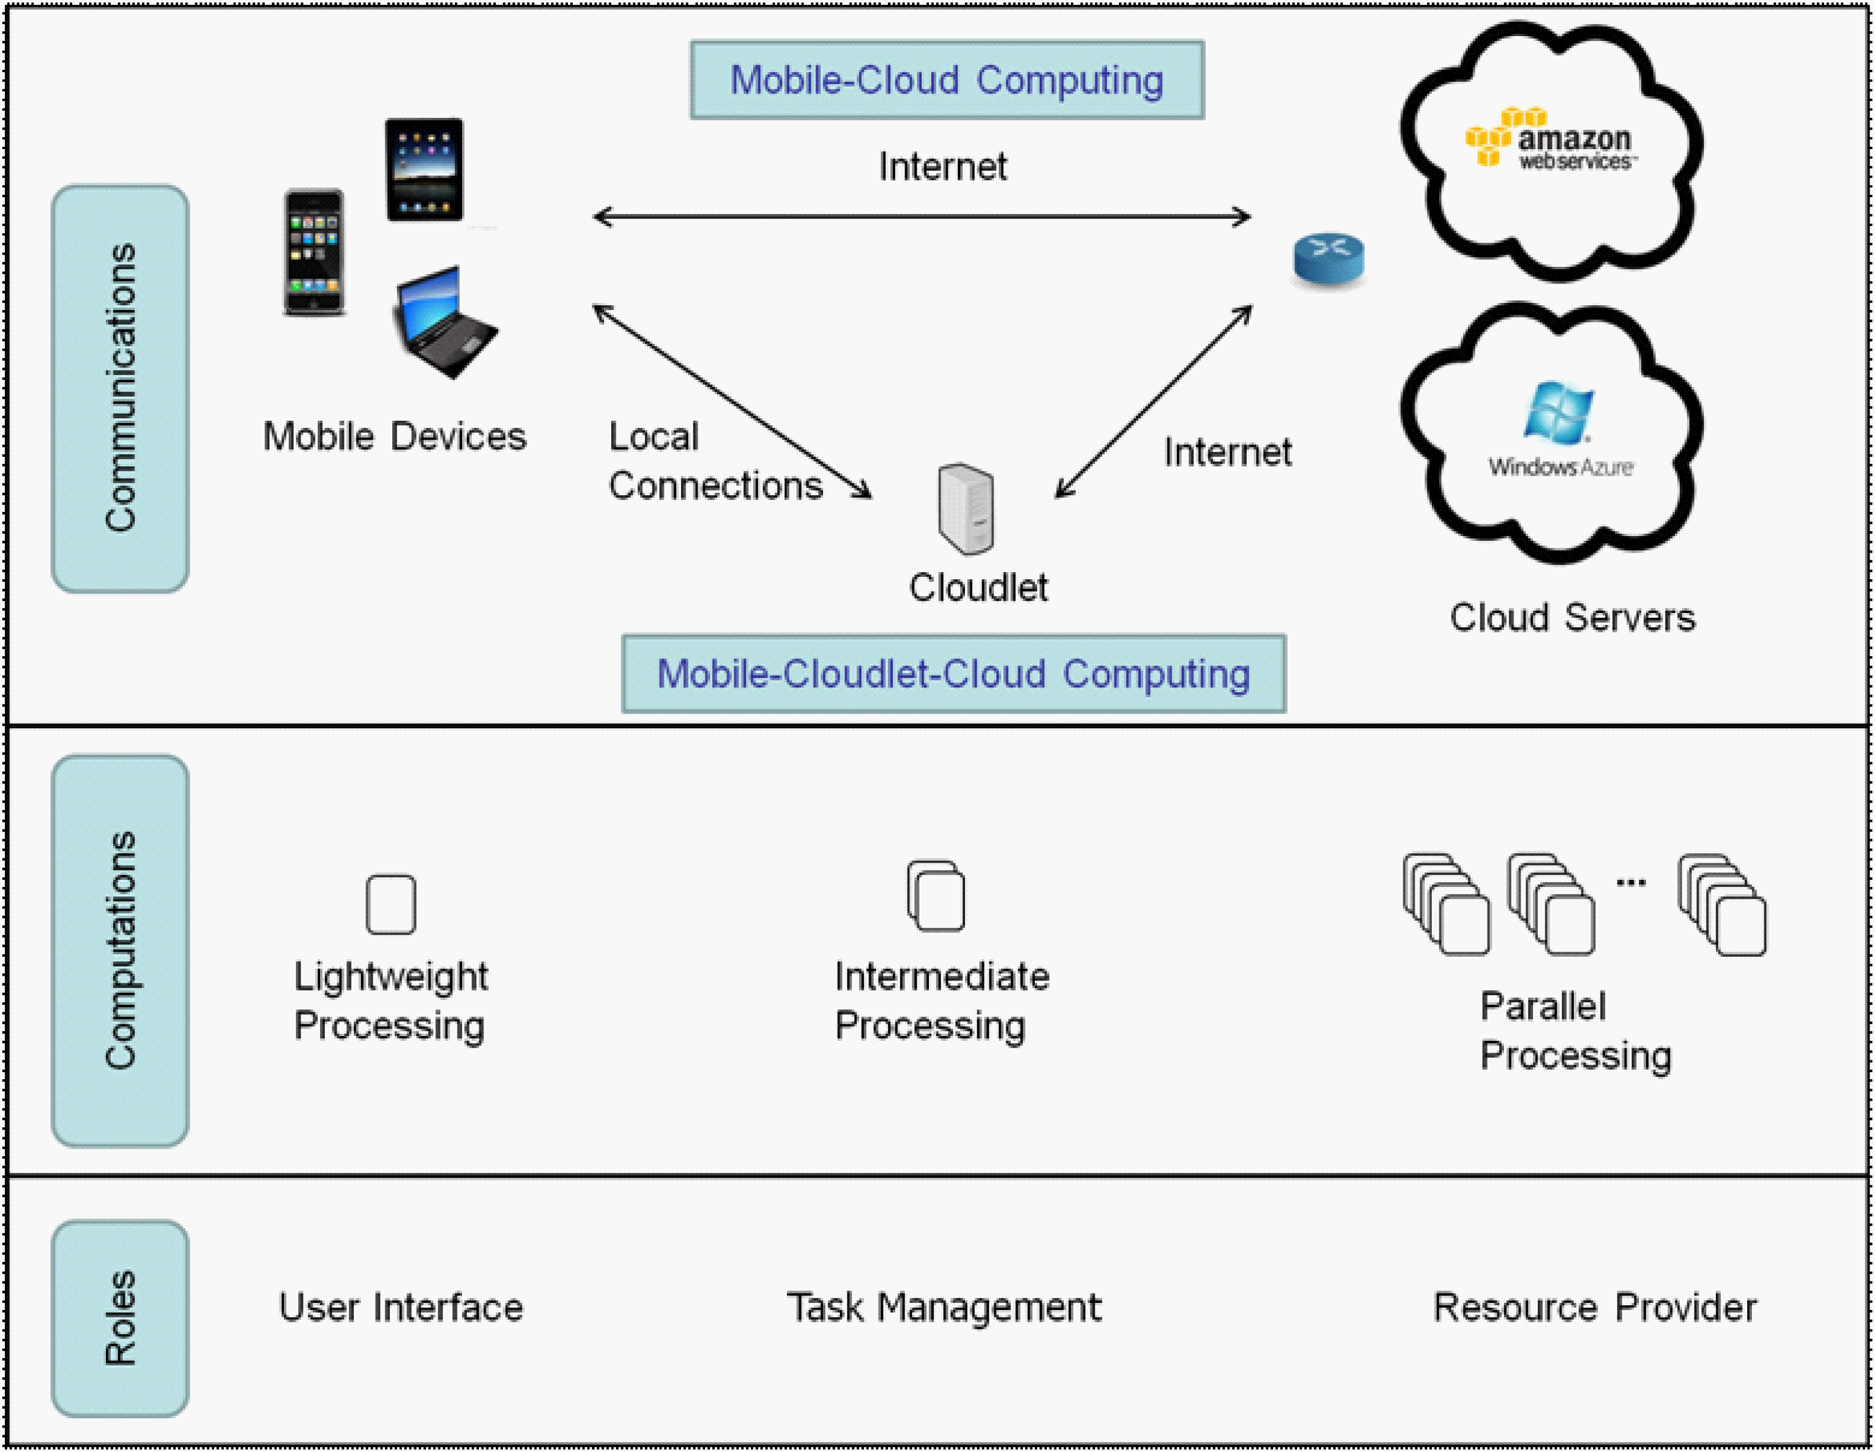
\includegraphics[scale=0.20]{Figures/mccarchitecturevscloudlet}
 \centering \caption{Diferencias entre las arquitecturas basadas en nube y las basadas en cloudlet \cite{soyata2013accelerating}}
 \label{fig:mccarchitecturevscloudlet}
\end{figure}

